\documentclass[a4,12pt]{article}
\usepackage[utf8]{inputenc} % para acentos y eñes
\usepackage[english,spanish]{babel}
\usepackage{verbatim} % para comentarios multilinea
\usepackage{graphicx} % para imagenes
\usepackage{hyperref}

% \usepackage{times} % tipo de letra de periodico
\renewcommand{\familydefault}{\sfdefault} % letras sin serifa

%opening
\title{Aplicación de la Geometría Proyectiva en Criptografía}
\author{Leandro J. Guillén Moreno}
\date{}

\begin{document}

\maketitle

\begin{abstract}
Historia de las curvas elípticas y la geometría proyectiva. Operaciones con puntos en curvas elípticas. Aplicación en la criptografía de las curvas elípticas.
\end{abstract}

\section{Curvas elípticas}


Una curva elíptica es una curva plana definida por una ecucación de la forma: $$y^{2}=x^{3}+ax+b$$ donde $a$ y $b$ son números reales. Este tipo de ecuación también es conocido como la \emph{Ecuación de Weierstrass}.

En las curvas elípticas se define un punto $O$, el cual representa el \emph{punto en el infinito} en el plano proyectivo.

Hola \cite{lamport94}.


\section{Correo de Leandro}
Correo recibido del profesor Leandro Marín

\begin{quotation}
Explicación de cómo funcionan las operaciones de puntos en curvas elípticas con todos los casos posibles (tangentes, punto del infinito, etc) con sus respectivos gráficos y luego completalo con algo que encuentres de la historia de las curvas elípticas y cómo se aplicaron a la criptografía. No es necesario mucho más y las 10 páginas las sacas enseguida.

Es una sugerencia, si no te gusta, buscamos algo diferente.
\end{quotation}
%%%%%%%%%%%%%%%%%%%%%%%%%%%%%%%%%%%%%%%%%%%%%%%%%%%
\section{Gráficos}

Para incluir una foto lo hacemos directamente. Ver el ejemplo de la imagen \ref{fig:monigote}.

\begin{figure}[h]
\begin{center}
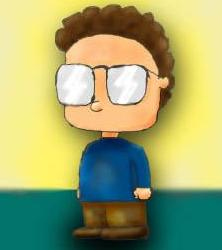
\includegraphics[width=0.2\linewidth]{imagenes/comic}
\end{center}
\caption{Un extraño monigote.}
\label{fig:monigote}
\end{figure}

\begin{figure}[h]
\begin{center}
\includegraphics[width=0.5\linewidth]{imagenes/dibujo}
\end{center}
\caption{Un dibujo vectorial hecho con Inkscape.}
\label{fig:monigote}
\end{figure}

Es más interesante introducir gráficos vectorizados.

%%%%%%%%%%%%%%%%%%%%%%%%%%%%%%%%%%%%%%%%%%%%%%%%%%%
\section{Tablas}

Las tablas se crean con el entorno \emph{tabular}. Se muestra un ejemplo en la tabla \ref{tab:resul}.

\begin{table}[h]
\begin{center}
\begin{tabular}{c|c|c} % las 3 columnas centradas (c) y con lineas entre ellas
\textbf{km} & \textbf{m} & \textbf{km/h} \\
\hline
\hline
1 & 2 & 3 \\
\hline
4 & 5 & 6 \\
\hline
7 & 8 & 9
\end{tabular}
\end{center}
\caption{Tabla de resultados.}
\label{tab:resul}
\end{table}

%%%%%%%%%%%%%%%%%%%%%%%%%%%%%%%%%%%%%%%%%%%%%%%%%%%
\section{Ecuaciones}

Tenemos tres tipos de ecuaciones.
\begin{enumerate}
\item En línea, como la siguiente $1+x_0=3^y-\alpha$.
\item El segundo tipo son las ecuaciones en su propio párrafo: $$1+x_0=3^y-\alpha$$
\item El tercer tipo de ecuaciones va numerado y podemos referenciarlo.
\begin{equation}\label{eq:gamma}
\beta^2=\frac{1}{\sqrt{1+x^2}}
\end{equation}

En otros lugares podemos referenciar ecuaciones, como la de arriba, que se llama \ref{eq:gamma}.

En las ecuaciones en su propio párrafo algunos elementos se ven más grandes. Ejemplo:
\begin{equation}\label{eq:absurda}
\pi^2-x=\sum_{k=0}^\infty \frac{1}{k^3}
\end{equation}
La expresión \ref{eq:absurda} es absurda.

\end{enumerate}

%%%%%%%%%%%%%%%%%%%%%%%%%%%%%%%%%%%%%%%%%%%%%%%%%%%
\section{Guión de \LaTeX}

\begin{enumerate}

\item Creamos un documento \texttt{.tex} mínimo y comprobamos que \texttt{pdflatex} funciona.

\item Creamos el archivo \texttt{Makefile} y configuramos el editor para quese grabe y recompile el documento automáticamente al pulsar un botón.

\item Añadimos el paquete \emph{imputenc} con la opción \texttt{[utf8]} para poder usar letras internacionales (con acentos, eñes, etc).

\item Creamos un entorno \emph{itemize} y \emph{enumerate}, y practicamos con texto enfatizado (cursiva) y de máquina de escribir \emph{textt}.

\item Los comentarios se indican con \verb+%+ (el resto de la linea, o con un entorno \emph{comment} proporcionado por el paquete \emph{verbatim}).

% Esto es un comentario
\begin{comment}
Esto es un comentario
de varias lineas.
\end{comment}

\item Creamos una sección con los pasos a seguir.

\item Ahora añadimos el título y el autor. Es necesario escribir \verb+\maketitle+ para que se muestre esta información. Si queremos eliminar la fecha ponemos \verb+\date{}+. Por defecto la fecha es \today (\verb+\today+).

\item Añadimos un resumen.

\item Cambiamos el ``idioma'' con el paquete \emph{babel}.

\item Cambiamos los tipos de letra y el tamaño base del documento.

\item No debemos abusar de los \textbf{cambios de tamaño}, pero es posible escribir {\scriptsize con letra pequeña} o {\huge muy grande}.

\item Ahora creamos una sección nueva para probar las ecuaciones.

\item Podemos cambiar a doble columna o la clase del documento.

\item Creamos tablas en una nueva sección. La centramos y la metemos en un entorno flotante.

\item Añadimos el índice.

\item Añadimos figuras y fotos.

\item Referencias bibliográficas. Puedo citar obras: Los estudios absurdos \cite{gomez98} han sido superados por trabajos recientes \cite{fernandez08}, lo que está muy mal.

\item A veces es útil usar el paquete \emph{hyperref}, que nos permite poner enlaces (\href{http://www.um.es}{Universidad de Murcia}).

\end{enumerate}

\bibliographystyle{plain}
\bibliography{refs} % mi archivo refs.bib
\end{document}
